\documentclass{article}
\usepackage[utf8]{inputenc}
\usepackage[a4paper, top=3cm, bottom=3cm, left=3cm, right=3cm]{geometry}
\usepackage{amsmath}
\usepackage{amsthm}
\usepackage{amssymb}
\usepackage{fancyhdr}
\usepackage{hyperref}
\usepackage{graphicx}
\usepackage{subfig}
\usepackage[T1]{fontenc}    % https://tex.stackexchange.com/questions/453540/
\usepackage{csquotes}       % https://www.overleaf.com/learn/latex/Typesetting_quotations

\pagestyle{fancy}
\fancyhf{}
\lhead{Competitive Programming}
\rhead{Week-1}
\cfoot{\thepage}

\newcommand{\B}[1]{\textbf{#1}}
\newcommand{\I}[1]{\textit{#1}}
\newcommand{\T}[1]{\texttt{#1}}
\newcommand{\Mod}[1]{\ (\mathrm{mod}\ #1)}

\title{\textbf{SoC 2023: Competitive Programming \\ {\Large Week-2: Sorting, Searching, and Number Theory}}}
\author{Mentor: Virendra Kabra}
\date{Summer 2023}

\begin{document}
\begin{sloppypar}       % for overfull, etc.

    \maketitle
    \tableofcontents
    \thispagestyle{empty}

    \newpage
    % \setcounter{page}{1}

    \section{Sorting}

    \subsection{C++}
    \begin{itemize}
        \item To sort vectors or strings, use \T{sort} from the STL. References: \href{https://www.geeksforgeeks.org/sort-c-stl/}{GFG}, \href{https://cplusplus.com/reference/algorithm/sort/}{cplusplus.com}.
        \item For $n$ items, number of operations is $O(n \log n)$.
        \item To sort a vector of custom structs, use a comparator function. Example in file.
    \end{itemize}

    \subsection{Algorithms}
    \begin{itemize}
        \item Comparison-based: Bubblesort $O(n^2)$, Mergesort $O(n\log n)$, Quicksort - average $O(n\log n)$, worst $O(n^2)$
        \item Counting sort: If all elements are in an interval of size $O(n)$, maintain a frequency array or \T{unordered\_map}, and finally list elements in order. Complexity $O(n)$.
    \end{itemize}

    \subsection{Examples}
    \begin{itemize}
        \item Find number of unique elements in an array. $O(n\log n)$ with sorting or \T{set}, $O(n)$ with \T{unordered\_set}.
        \item Interval scheduling. Given a list of intervals with respective start and end times, report the maximum number of non-overlapping intervals.
        \begin{center}
            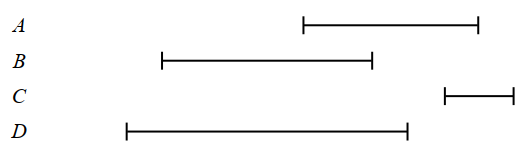
\includegraphics[width = 0.9\linewidth]{../images/interval-sched.png}
        \end{center}
        Here, $\{B,C\}$ or $\{D,C\}$ are optimal. $\{A,C\}$ is not valid, while $\{A\}$ is sub-optimal.

        \noindent A ``greedy'' solution: always choose the next interval with smallest finish time (this requires sorting). The algorithm is greedy in the sense of local optimization. It is also globally optimal: for any schedule that you pick, we can replace the first interval with an interval that ends earlier and repeat the process.

        \item Find the maximum number of overlapping intervals: Sort all start and end times in a single vector, with information if it is start/end. Iterate over and maintain a counter: $+1$ for start, $-1$ for end. Max counter value is the answer.
    \end{itemize}

    \newpage

    \section{Binary Search}
    \subsection{Introduction}
    \begin{itemize}
        \item Search for an element in a \B{sorted} array. Search range halves in every iteration, so going from space of size $n$ to that of size $1$ takes $O(\log_2 n)$ iterations.
        \begin{center}
            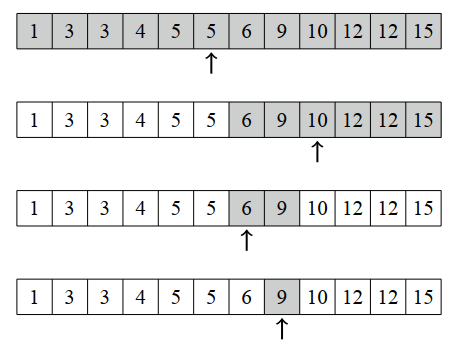
\includegraphics[width = 0.5\linewidth]{../images/bin-search.png}
        \end{center}
        \item Code in file.
    \end{itemize}

    \subsection{Examples}
    \begin{itemize}
        \item Find the maximum value in a unimodal array. Use the interval-halving idea with a different condition.
        \begin{center}
            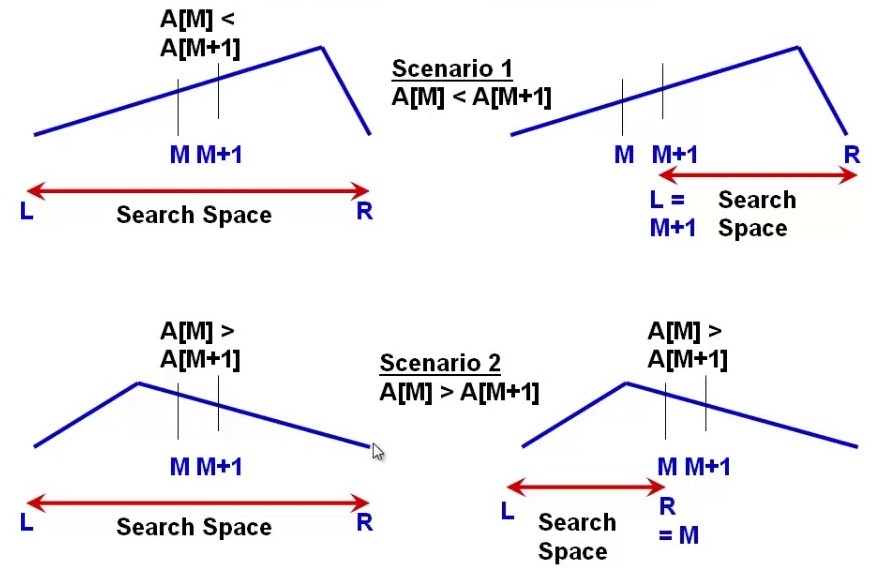
\includegraphics[width = 0.8\linewidth]{../images/unimodal.jpg}
        \end{center}
        \item \href{https://www.geeksforgeeks.org/the-painters-partition-problem-using-binary-search/}{Painters' Partition Problem}
        \begin{displayquote}
            We have to paint $n$ boards of lengths $\{A_1, A_2, \dots, A_n\}$. $k$ painters are available and each takes $1$ unit time to paint $1$ unit of board. Find the minimum time to get the job done under the constraint that any painter will only paint continuous sections of boards.\\
            Example: Lengths $\{9, 4, 7, 10, 5\}$ with $k=3$. Allocations $\{9\}, \{4, 7\}, \{10, 5\}$ and $\{9, 4\}, \{7\}, \{10, 5\}$ are optimal, while $\{9, 4\}, \{7, 10\}, \{5\}$ isn't.
        \end{displayquote}
        Maximum time taken by any painter is the answer. Assuming any number of painters, an initial \I{range} on this is $\big[\max_{i} A_i,\sum_{i}A_i\big]$ - with $n$ and $1$ painters respectively.\\
        A number $t$ is a candidate answer if we can assign contiguous segments to $\le k$ painters, each of length $\le t$. If $t$ works, then any number $\ge t$ works. So, we have an array like the following
        \begin{center}
            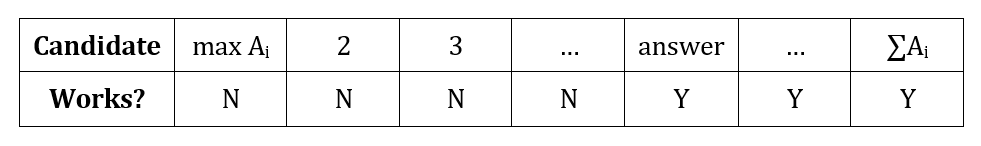
\includegraphics[width = 0.8\linewidth]{../images/painter.png}
        \end{center}
        Candidates are sorted, so we can use binary search. To check if a candidate works, need to iterate over the array in $O(n)$. The overall complexity is $O(n\log (\sum A_i - \max{A_i}))$.

        \noindent Code in file. We can start with a much larger initial interval such as $[0,\text{INT\_MAX}]$; idea remains the same.
    \end{itemize}

    \newpage

    \section{Number Theory}

    \subsection{Factors}
    \begin{itemize}
        \item Factors of a number $n$: Iterate from $1$ to $\sqrt{n}$. If \T{n\%i == 0}, then $i$ and $n/i$ are factors.
        \item Primes: \href{https://cp-algorithms.com/algebra/sieve-of-eratosthenes.html}{Sieve of Eratosthenes}. For example, we need primes from $L$ to $R$. Check the reference for a simple \href{https://cp-algorithms.com/algebra/sieve-of-eratosthenes.html#implementation}{implementation}.
        \begin{center}
            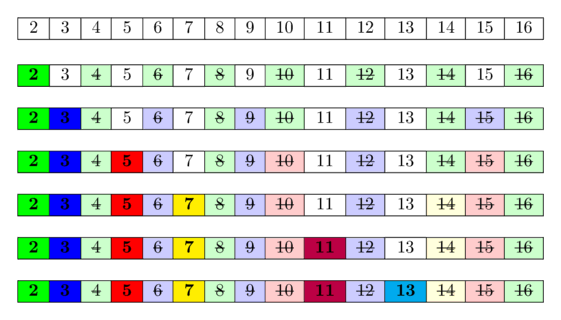
\includegraphics[width = 0.8\linewidth]{../images/sieve_eratosthenes.png}
        \end{center}
        \item Prime decomposition of $n$: Use the sieve to get primes in $[2, \sqrt{n}]$ and test with each prime. \href{https://cp-algorithms.com/algebra/factorization.html#precomputed-primes}{Implementation}.
    \end{itemize}

    \subsection{Combinatorics}
    \begin{itemize}
        \item Modular arithmetic: $a \equiv (a\%m) \Mod{m}$. $m$ is usually a large prime to ease later calculations.
        \item Binary exponentiation: $a^b \Mod{m}$ in $O(\log_2 b)$. Code in file.
        \item Inverse Modulo: With Euler's Totient function $\phi$, $a^{\phi(m)} \equiv 1 \Mod{m}$. For prime $m$, this is $a^{m-1} \equiv 1 \Mod{m}$. Further, if $\gcd{(a,m)} = 1$, we get $a^{m-2} \equiv a^{-1} \Mod{m}$.\\
        So $a^{-1} \Mod{m}$ is equivalent to $a^{m-2}\%m$ - use binary exponentiation.
        \item ${n \choose k} = \frac{n!}{k!(n-k)!}$. Modulo prime $m$, we use precomputed factorials and inverse modulo.
        \item Resources: \href{https://cp-algorithms.com/algebra/binary-exp.html}{Binary Exponentiation}, \href{https://cp-algorithms.com/algebra/module-inverse.html#definition}{Modular Inverse}, \href{https://cp-algorithms.com/combinatorics/binomial-coefficients.html#computing-binomial-coefficients-modulo-m}{Binomial Coefficients}
    \end{itemize}

    \section{Todos}
    \begin{itemize}
        \item First 5 problems from CSES (Sorting and Searching)
        \item Codeforces: 1612C, 1613C, 1610C
    \end{itemize}

\end{sloppypar}
\end{document}